\section{No algorithm for \prob{IndependentSet}/\td{} under SETH}
\label{section:indset-td}

Esmer et al. \cite{esmer2024fundamental} demonstrated that there is no $\varepsilon > 0$ such that there is an algorithm running in time $\O^\star((2 - \varepsilon)^\td)$ for $\prob{IndependentSet}/\td$ without contradicting SETH, as shown in \refcorollary{corollary:td-lowerbounds}. However, we have discovered an alternative method to arrive at the same result, which we will describe in this section.

\medskip

Let $\phi$ be an instance of SAT with $n$ variables and $m$ clauses. The main idea of the proof is to create a graph $G$ with an elimination forest of size approximately $n$. This graph $G$ is constructed such that any independent set of $G$ corresponds to an assignment of variables in $\phi$. If $\phi$ is satisfiable, then the largest independent set in $G$ will have size $k$, where $k$ depends on $\phi$. Conversely, if $\phi$ is not satisfiable, no independent set of size $k$ can be found. Thus, finding an $\O^\star((2 - \varepsilon)^\td)$ for \prob{IndependentSet} would imply the existence of a similar algorithm for \prob{SAT}, contradicting SETH. Let us now prove this formally.

\begin{theorem}
    \label{theorem:indset-td-lowerbound}
    Given $\varepsilon > 0$, if \prob{IndependentSet} can be solved in time $\O^\star((2-\varepsilon)^\td)$, then \prob{SAT} can be solved in time $\O^\star((2 - \delta)^n)$ for some $\delta > 0$.
\end{theorem}

\paragraph*{Construction of $G$} Given $0 < \varepsilon < 1$ and an instance of $\phi$ of SAT, we construct a graph $G$ as follows. First, we choose an even integer $p$ depending only on $\varepsilon$; the value of this constant will be discussed later. We partition the variables of $\phi$ into groups $V_1, \dots, V_t$, each containing at most $\beta = \left\lfloor\log\binom{p}{p/2}\right\rfloor$ variables. Note that $t = \left\lceil n/\beta\right\rceil$.

\medskip

\begin{figure}
    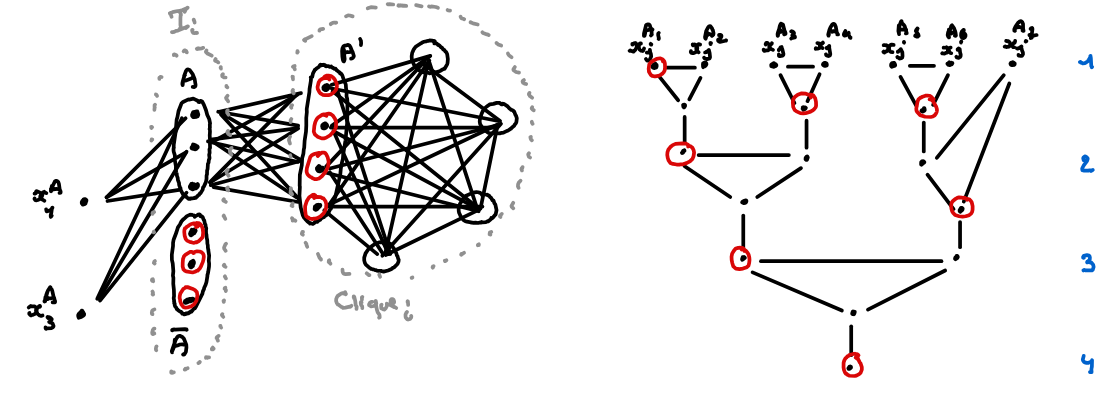
\includegraphics[width=\textwidth]{figures/indset-td-gadgets.png}
    \caption{Reduction from SAT to \prob{IndependentSet}: on the left, a group gadget for $p = 6$, for readability, only one pair $(A, A')$ has been depicted, but there are $\binom{6}{3} = 20$ such pair $(A, A')$. The assignment associate to $A$ satisfies clauses $c_1$ and $c_3$. On the right, a clause gadget with 7 assignments validating $c_j$, in blue we have shown the depth of the vertices during the construction of the gadget. One best independent set has been shown in red for both gadgets.}
    \label{fig:indset-td-gadgets}
\end{figure}

Now, let us describe the construction of a \textit{group gadget} $G_i$, for a given group $V_i$ (see \reffigure{fig:indset-td-gadgets}):

\begin{enumerate}
    \item Introduce a set $I_i$ of $p$ independent vertices.
    \item For each subset $A \subseteq I_i$ containing exactly $\frac{p}{2}$ vertices, construct a corresponding group $A'$ consisting of $\frac{p}{2} + 1$ vertices. By $\bar{A}$, we denote $I_i - A$.
    \item Connect $A$ and $A'$ as a complete bipartite graph. This configuration ensures that if any vertex from $A$ is included in an independent set of $G_i$, then none of the vertices from $A'$ can be included, and vice versa.
    \item Connect all $A'$ groups together in a clique manner. This setup ensures that if any vertex from one $A'$ group is included in an independent set of $G_i$, then no vertex can be included fro any other $A'$ group. By $Clique_i$, we denote the union of all $A'$.
\end{enumerate}

\medskip

For each $1 \leq i \leq t$ and every assignment of variables of the group $V_i$, we associate a subset $A \subseteq I_i$ consisting of exactly $\frac{p}{2}$ vertices. Given that there are at most $2^\beta$ different assignments for the variables in $V_i$, and since $\binom{p}{p/2} \geq 2^\beta$, there exists a unique subset $A$ corresponding to each assignment.

\medskip

Now, let us describe the construction of a \textit{clause gadget} $C_j$, for a given clause $c_j$ of $\phi$, (see \reffigure{fig:indset-td-gadgets}):
\begin{enumerate}
    \item For each group variable $V_i$ and for every assignment of $V_i$ that satisfies $c_j$, let $A$ denote the associated set of vertices in the group gadget $G_i$. Create a vertex $x_j^A$ and connect it to every vertices of $A$.
    \item Let $X$ denote the set of all $x_j^A$ vertices created for clause $c_j$. Initially, assign each vertex in $X$ a depth of 1. Construct the gadget $C_j$ through the following steps until $X$ contains only one vertex:
    \begin{itemize}
        \item Remove the two vertices from $X$ with the smallest depth $x_1$ (depth $d_1$) and $x_2$ (depth $d_2$).
        \item Introduce a new vertex $y$ and form a triangle connecting $y$, $x_1$ and $x_2$.
        \item Introduce a new vertex $z$ and connect $y$ to $z$.
        \item Add $z$ to $X$ and assign it a depth of $\max(d_1, d_2) + 1$. 
    \end{itemize}
\end{enumerate}

\medskip

This ends the construction of $G$.

\begin{lemma}
    \label{lemma:group-gadget-indset}
    The largest independent set in a group gadget $G_i$ has size $p+1$. Moreover, each independent set of size $p+1$ consists of $\bar{A} \cup A'$ for one $A \subseteq I_i$.
\end{lemma}

\begin{proof}
    Suppose $\I$ an independent set of max size of $G_i$.
    \begin{itemize}
        \item \textbf{Case 1:} There is at least one vertex $x \in \I \cap Clique_i$. Let $A'$ be the group containing $x$. By construction, $x$ is connected to all vertices in $Clique_i - A'$. Moreover, $x$ is also connected to every vertex in $A \subseteq I$ associated with $A'$. The only possible vertices remaining are those from $A'$ and $\bar{A}$, which forms an independent set. Thus, by maximality of $\I$, we know $\I = A \cup \bar{A}$.
        \item \textbf{Case 2:} $\I \cap Clique_i = \emptyset$. In this case, only the vertices of $I_i$ remain, and there are only $p$ vertices in $I_i$. Thus $\I$ cannot be larger than $p$ vertices.
    \end{itemize}

    \medskip

    Therefore, the largest independent set in $G_i$ has size $p+1$, and each such independent set consists of $\bar{A} \cup A'$ for som $A \subseteq I$.
\end{proof}

\begin{lemma}
    \label{lemma:clause-gadget-indset}
    The largest independent set in a clause gadget $C_j$ has size $\alpha_j$ where $\alpha_j$ corresponds to the number of different assignments from $V_i$ satisfying $c_j$. Moreover, each independent set of size $\alpha_j$ contains at least one $x_j^A$. Finally, having only one $x_j^A$ suffices to form an independent set of size $\alpha_j$.
\end{lemma}

\begin{proof}
    Suppose $\I$ an independent set of max size of $C_j$.
    \begin{itemize}
        \item \textbf{Case 1:} No $x_j^A \in \I$. According to the construction of $C_j$, if no $x_j^A$ is in $\I$, then the remaining of $C_j$ consists of $\alpha_j - 1$ cliques of size $2$ (see \reffigure{fig:indset-td-best}). Therefore, the maximum size of the independent set $\I$ would be $\alpha_j - 1$.
        \item \textbf{Case 2:} At least one $x_j^A \in \I$. In this scenario, $C_j$ can be partitioned into $\alpha_j$ cliques (see \reffigure{fig:indset-td-best}): $\alpha_j - 1$ triangles and one additional vertex at the bottom. To find the largest independent set, we proceed in a bottom-up manner:
        \begin{itemize}
            \item Mark a triangle has \textit{good} if at least one of its top vertices ($x_1$ or $x_2$) is in $\I$.
            \item For $\I$ to be of size $\alpha_j$, the bottom vertex must be in $\I$, which forces the triangle directly above it to be good.
            \item Assume the vertex in $\I$ from the triangle directly above the bottom vertex is the upper left one. This forces the triangle above it to be good, and so on, up to the top most triangles. Note that in this case, the triangle above the upper right vertex doesn't need to be good.
            \item At least one top triangle must be good, meaning at least one $x_j^A \in \I$.
        \end{itemize}
        
        \medskip
        
        Note that only one top triangle needs to be good, so having just one $x_j^A \in \I$ is sufficient to form an independent set of size $\alpha_j$.
        
        \medskip

        Therefore, the largest independent set in $C_j$ has size $\alpha_j$, and each independent set of this size contains at least one $x_j^A$. Having only one $x_j^A$ suffices to form an independent set of size $\alpha_j$.
    \end{itemize}
\end{proof}

\begin{figure}
    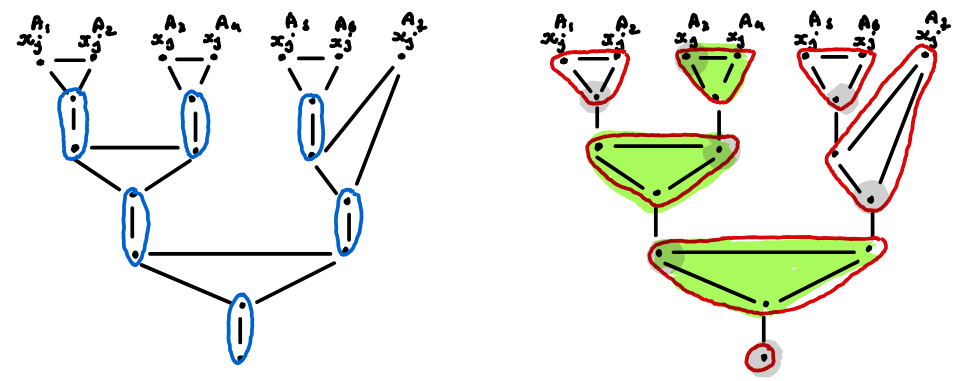
\includegraphics[width=\textwidth]{figures/indset-td-best.png}
    \caption{Finding the largest independent set $\I$ of a clause gadget $C_j$. On the left, the case where no $x_j^A$ are allowed in $\I$. The cliques are shown in blue. On the right, the case where $x_j^A$ can be in $\I$. The cliques are shown in red. An example of an independent set of size $\alpha_j$ is shown in gray, with the \textit{good} triangles highlighted in green.}
    \label{fig:indset-td-best}
\end{figure}

\begin{lemma}
    \label{lemma:indset-sat-graph-equiv}
    The formula $\phi$ is satisfiable if and only if $G$ has an independent set of size $t(p+1) + \sum_{i = 1}^j \alpha_j$.
\end{lemma}

\begin{proof}
    \begin{itemize}
        \item [$\Rightarrow$] Suppose $\pazocal{A}$ an assignment of variables that satisfies $\phi$. We will construct an independent set $\I$.
        
        For each group $V_i$:
        \begin{itemize}
            \item Consider the part $\pazocal{A}_i$ of the assignment $\pazocal{A}$ that contains the variable of $V_i$. Let $A_i$ be the set of vertices in the group gadget $G_i$ associated with $\pazocal{A}_i$.
            \item According to \reflemma{lemma:group-gadget-indset}, we can take $\bar{A_i} \cup A_i'$ inside $\I$.
        \end{itemize}
        For each clause gadget $C_j$:
        \begin{itemize}
            \item There is an assignment of a variable in $\pazocal{A}$ that satisfies the clause $c_j$, suppose this variable is in group $V_i$.
            \item We have currently $\bar{A_i}$ in $\I$, and the vertices of $A_i$ are not included in $\I$.
            \item Thus we can include $x_j^{A_i}$ in $\I$. According to \reflemma{lemma:clause-gadget-indset}, we can form an independent set of size $\alpha_j$ for $C_j$, which we add to $\I$.
        \end{itemize}
        
        \medskip

        The total size of $\I$ is $p+1$ for each group gadget and $\alpha_j$ for every clause gadget $C_j$, resulting in a total size of $t(p+1) + \sum_{i = 1}^j \alpha_j$.

        \item [$\Leftarrow$] Suppose there is an independent set $\I$ of size $t(p+1) + \sum_{i = 1}^j \alpha_j$. By combining \reflemma{lemma:group-gadget-indset} and \reflemma{lemma:clause-gadget-indset}, we know that $\I$ has a specific structure:
        
        \begin{itemize}
            \item For each group gadget $G_i$, there is an $A_i$ such that $\I \cap G_i = \bar{A_i} \cup A_i'$.
            \item For each clause gadget $C_j$, there exists a $x_j^A \in \I$.
        \end{itemize}

        We assign the variables of $V_i$ according to the assignment associated with $A_i$. If no assignment is associated to $A_i$, we choose any assignment for the variables of $V_i$.
        
        Every clause is satisfied by our assignment of variables. Specifically, if $x_j^A \in I$ for the clause gadget $C_j$, it means no vertices from $A$ are in $\I$. Therefore,the assignment chosen for the variables in $V_i$ satisfies the clause $c_j$ by construction of $C_j$.
    \end{itemize}
\end{proof}

\begin{lemma}
    \label{lemma:indset-sat-graph-td}
    The treedepth of $G$ is at most $tp + \O(\log n) + f(p)$ for $f$ some function depending on $p$.
\end{lemma}

\begin{proof}
    We will construct an elimination forest $\F$ for the graph $G$. This elimination forest is depicted in \reffigure{fig:indset-elimination-forest}.
    
    \begin{itemize}
        \item First, consider every vertex in each $I_i$ of all $G_i$ as forming a trunk of size $tp$ in $\F$.
        \item  Each $Clique_i$ in $G_i$ contains $(p+1)\binom{p}{p/2}$ vertices. Thus $G_i$ has a treedepth of at most $(p+1)\binom{p}{p/2}$.
        \item Moreover, these cliques only connect to vertices in $I_i$, so multiple $Clique_i$ does not increase the depth of $\F$.
        \item Each clause gadget $C_j$ can be decomposed into a tree structure. The bottom vertex represent the root and each triangle in the gadget can be viewed as an internal node with three vertices.
        \item This forms a binary tree with $\alpha_j$ leaves, giving it a depth of $\lceil3\log{\alpha_j}\rceil$. Since $\alpha_j \leq t\binom{p}{p/2}$, the depth is $\O(\log(t\binom{p}{p/2}))$ for $C_j$.
        \item Because $C_j$ only connects to vertices in $I_i$, adding multiple clause gadgets does not increase the depth of $\F$.
    \end{itemize}

    \medskip

    By combining these components, the total treedepth of $G$ is at most $tp + \O(\log n) + f(p)$. The detailed computation can be found in \refappendix{appendix:boring-proofs}.
\end{proof}

\begin{figure}
    \centering
    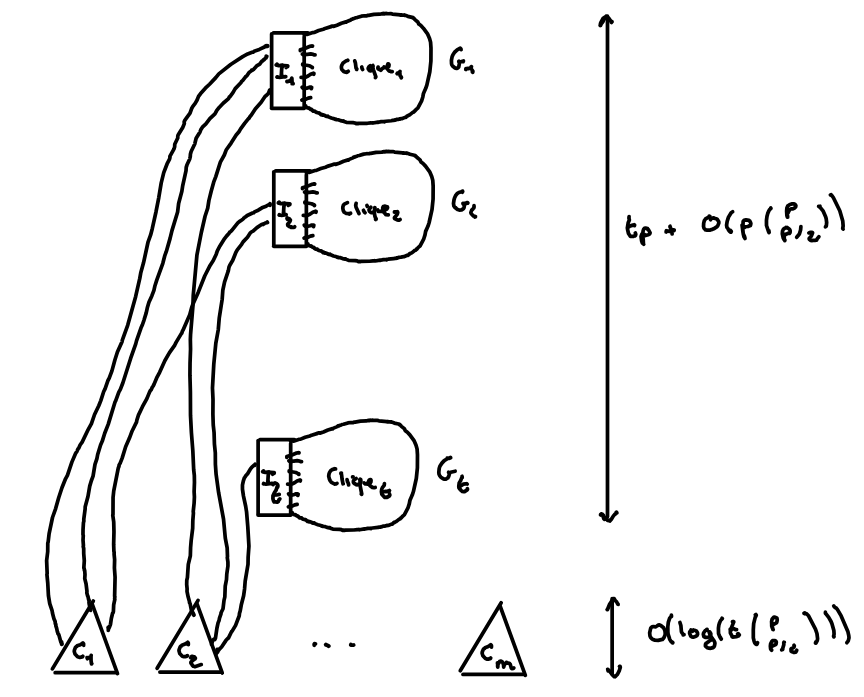
\includegraphics[width=.6\textwidth]{figures/indset-elimination-forest.png}
    \caption{An elimination forest of $G$.}
    \label{fig:indset-elimination-forest}
\end{figure}

Now we are ready to prove \reftheorem{theorem:indset-td-lowerbound}.

\begin{proof}
    (of \reftheorem{theorem:indset-td-lowerbound}). Suppose $\prob{IndependentSet}/\td$ can be solved in $\O^\star((2-\varepsilon)^\td)$. We fix $\lambda > 0$ such that $(2 - \varepsilon)^{1 + \lambda} \leq 2 - \frac{\varepsilon}{2}$; note that such a $\lambda$ always exists and depends only on $\varepsilon$. Next, we choose $p \geq 2$ such that $p/(p - \frac{1}{2} + \frac{1}{2}\log(\pi p)) \leq 1 + \lambda$. This is feasible since the limit to infinity of the left part is 1. Moreover $p$ only depends on $\varepsilon$. 
    
    Given an instance of \prob{SAT}, we construct an instance of $\prob{IndependentSet}$ using the above construction and the chosen value of $p$. Then we solve the $\prob{IndependentSet}$ instance using the $\O^\star((2 - \varepsilon)^\td)$ time algorithm. Corectness is ensured by \reflemma{lemma:indset-sat-graph-equiv}. \reflemma{lemma:indset-sat-graph-td} yields that the total time taken is upper bounded by: $$\O^\star((2-\varepsilon)^{tp + \O(\log n) + f(p)}) = \O^\star((2-\varepsilon)^{tp}) \leq \O^\star((2-\frac{\varepsilon}{2})^{n})$$ due to our choice of $p$. To see the full computation, please refer to \refappendix{appendix:boring-proofs}. By saying $\delta = \frac{\varepsilon}{2}$, we have proven \reftheorem{theorem:indset-td-lowerbound}.
\end{proof}

Therefore, no such algorithm exists for $\prob{IndependentSet}/\td$ or the SETH fails.